%% Compiles the four TikZ figures of the paper:
%%   pdflatex tikz_figures.tex
%% The figure files are the same ones the paper inputs. Citations in captions
%% are replaced by plain brackets so that no bibliography is needed.
\documentclass[a4paper,11pt]{article}
\usepackage[margin=2cm]{geometry}
\usepackage{amsmath,amssymb}
\usepackage{xcolor}
\usepackage{float}
\usepackage{caption}
\usepackage{tikz}
\usetikzlibrary{positioning,arrows.meta,shapes.geometric,calc,fit,backgrounds}

\newcommand{\vmax}{v_{\max}}
\newcommand{\vmin}{v_{\min}}
\newcommand{\citep}[1]{[#1]}
\newcommand{\citet}[1]{[#1]}

% palette shared with scripts/gen_figures.py
\definecolor{NavyHeader}{RGB}{31,56,100}
\definecolor{NavyLight}{RGB}{217,225,242}
\definecolor{BrickRed}{RGB}{178,58,72}
\definecolor{SeaTeal}{RGB}{60,141,122}
\definecolor{VarTTP1}{HTML}{8DA0CB}
\definecolor{VarPWT}{HTML}{66C2A5}
\definecolor{VarTTP2}{HTML}{FC8D62}
\definecolor{VarMTTP}{HTML}{FFD92F}
\definecolor{VarDTTP}{HTML}{A6D854}
\definecolor{VarThOP}{HTML}{7FCDCD}
\definecolor{VarTTPTW}{HTML}{E78AC3}
\definecolor{VarCCTTP}{HTML}{B399D4}
\definecolor{VarTTPD}{HTML}{E5998F}
\definecolor{FigAmber}{HTML}{F0C239}
\definecolor{FigGrayBg}{HTML}{F1F3F5}

\begin{document}
% Schematic: the tour--packing feedback loop that defines the TTP.
\begin{figure}[H]
\centering
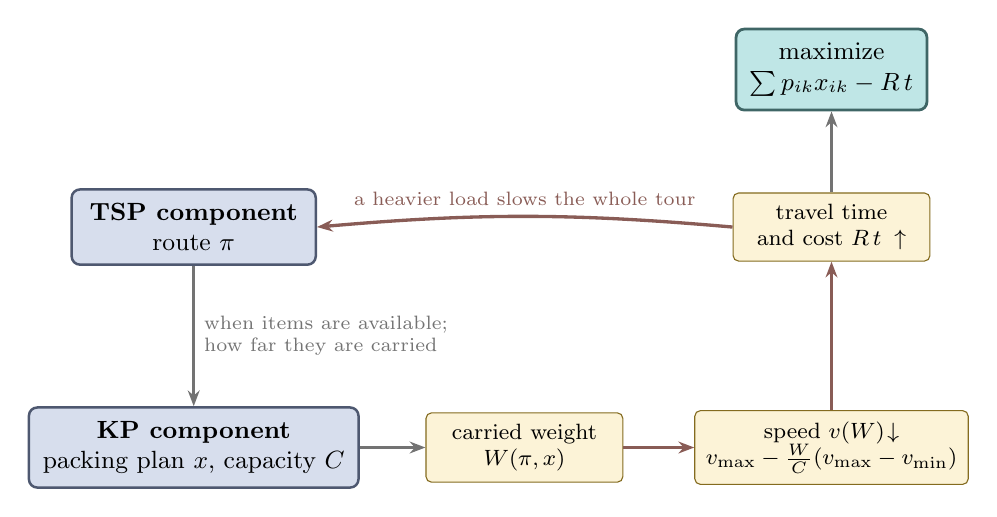
\begin{tikzpicture}[
  font=\small, >={Stealth[length=2mm]},
  comp/.style={draw=VarTTP1!55!black,line width=0.9pt,fill=VarTTP1!35,
               rounded corners=3pt,align=center,inner sep=5pt,minimum width=3.1cm},
  stp/.style={draw=FigAmber!55!black,fill=FigAmber!20,rounded corners=2pt,align=center,
               inner sep=4pt,font=\footnotesize,minimum width=2.5cm},
  obj/.style={draw=VarThOP!50!black,line width=1pt,fill=VarThOP!50,text=black,
              rounded corners=3pt,align=center,inner sep=5pt},
  k/.style={->,line width=0.9pt,black!55},
  fk/.style={->,line width=1.2pt,VarTTPD!60!black},
]
\node[comp] (tsp) at (0,1.4)  {\textbf{TSP component}\\route $\pi$};
\node[comp] (kp)  at (0,-1.4) {\textbf{KP component}\\packing plan $x$, capacity $C$};
\node[stp] (w)  at (4.2,-1.4) {carried weight\\$W(\pi,x)$};
\node[stp] (v)  at (8.1,-1.4) {speed $v(W)\!\downarrow$\\$\vmax-\tfrac{W}{C}(\vmax-\vmin)$};
\node[stp] (t)  at (8.1,1.4)  {travel time\\and cost $R\,t\;\uparrow$};
\node[obj]  (g)  at (8.1,3.4)  {maximize\\$\sum p_{ik}x_{ik}-R\,t$};

\draw[k] (tsp) -- node[right,align=left,font=\scriptsize,text=black!55]
  {when items are available;\\how far they are carried} (kp);
\draw[k] (kp) -- (w);
\draw[fk] (w) -- (v);
\draw[fk] (v) -- (t);
\draw[k]  (t) -- (g);
\draw[fk] (t.west) to[out=175,in=5] node[above,align=center,font=\scriptsize,text=VarTTPD!60!black]
  {a heavier load slows the whole tour} (tsp.east);
\end{tikzpicture}
\caption{Anatomy of the Traveling Thief Problem: the tour--packing feedback loop.}
\label{fig:anatomy}
\end{figure}

% PRISMA 2020 study-selection flow. All counts are exact, from the logged
% search of Scopus and Web of Science on 5 September 2026 (Section 2.2),
% plus a supplementary, non-exhaustive Google Scholar pass for preprints not
% indexed by either database.
\newcommand{\nScopus}{450}     % Scopus, raw query, no database-level filter
\newcommand{\nWoS}{670}        % Web of Science, raw query, no database-level filter
\newcommand{\nUnion}{1{,}120}  % records identified, Scopus + Web of Science
\newcommand{\nDup}{439}        % duplicate records removed
\newcommand{\nScreened}{681}   % records screened after duplicate removal
\newcommand{\nExclScreen}{594} % excluded at screening
\newcommand{\nRemain}{87}      % records retained after screening (before Google Scholar)
\newcommand{\nGS}{15}          % records added via Google Scholar (other methods)
\newcommand{\nCombined}{102}   % reports assessed for eligibility, \nRemain + \nGS
\newcommand{\nExclFTa}{7}      % excluded: theses
\newcommand{\nExclFTb}{1}      % excluded: short abstract with no model

\begin{figure}[htbp]
\centering
\begin{tikzpicture}[
  font=\footnotesize,
  >={Stealth[length=2mm]},
  node distance=0.6cm,
  box/.style={draw=VarTTP1!55!black,line width=0.7pt,fill=VarTTP1!30,
              align=center,inner sep=5pt,text width=5.2cm,rounded corners=2pt},
  other/.style={draw=VarThOP!55!black,line width=0.7pt,fill=VarThOP!25,
              align=center,inner sep=5pt,text width=3.6cm,rounded corners=2pt},
  exc/.style={draw=FigAmber!55!black,line width=0.6pt,fill=FigAmber!18,align=left,
              inner sep=4pt,text width=3.6cm,rounded corners=2pt,font=\scriptsize},
  inc/.style={draw=VarThOP!50!black,line width=0.9pt,fill=VarThOP!50,text=black,
              align=center,inner sep=5pt,text width=5.2cm,rounded corners=2pt},
  a/.style={->,line width=0.8pt,black!55},
]
\node[box] (id)
  {\textbf{Identification.} Records identified from two databases,
   searched 5 September 2026\\[2pt]
   \scriptsize Scopus (n=\nScopus), Web of Science (n=\nWoS)\\[2pt]
   Combined\ \ \textbf{n=\nUnion}};
\node[box,below=of id] (dedup)
  {Records screened after duplicate removal\ \ \textbf{n=\nScreened}};
\node[box,below=1.0cm of dedup] (screen)
  {\textbf{Screening.} Records retained after screening\ \ \textbf{n=\nRemain}};
\node[box,below=1.2cm of screen] (combined)
  {Reports assessed for eligibility\ \ \textbf{n=\nCombined}};
\node[inc,below=1.0cm of combined] (final)
  {\textbf{Included.} Studies in the review\ \ \textbf{94}\\
   \scriptsize 93 primary studies $+$ 1 prior systematic survey};

\node[other,left=0.9cm of combined] (other)
  {\textbf{Identified via other methods.} Google Scholar, preprints not
   indexed by either database\ \ \textbf{n=\nGS}};

\node[exc,right=0.5cm of dedup] (e1)
  {\textbf{n=\nDup} duplicate records removed};
\node[exc,right=0.5cm of screen] (e2)
  {\textbf{n=\nExclScreen} excluded at screening: off-topic, including the
   TTP used only as a minor example; not in English; outside January 2013 to
   September 2026; an excluded document type; or a short abstract with no
   model};
\node[exc,right=0.5cm of final] (e3)
  {\textbf{n=8} excluded after combining the two streams: theses
   (n=\nExclFTa); short abstract with no model (n=\nExclFTb)};

\draw[a] (id) -- (dedup);
\draw[a] (dedup) -- (screen);
\draw[a] (screen) -- (combined);
\draw[a] (other) -- (combined);
\draw[a] (combined) -- (final);
\draw[a] (dedup.east) -- (e1.west);
\draw[a] (screen.east) -- (e2.west);
\draw[a] (final.east)  -- (e3.west);
\end{tikzpicture}
\caption{Study selection following the PRISMA~2020 statement \citep{page2021prisma}.}
\label{fig:prisma}
\end{figure}

% Schematic: the TTP variant design space as a directed acyclic graph.
\begin{figure}[H]
\centering
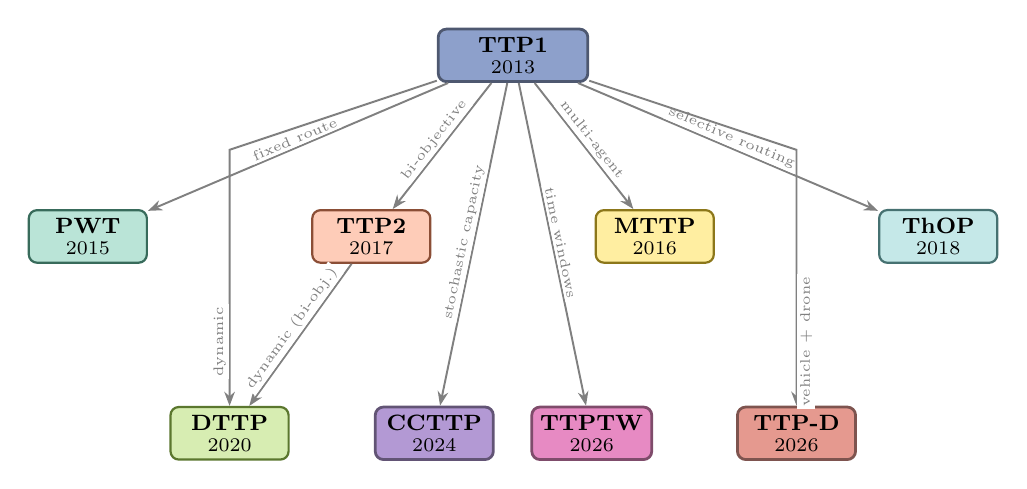
\begin{tikzpicture}[
  font=\footnotesize, >={Stealth[length=1.8mm]},
  root/.style={draw=VarTTP1!55!black,line width=1pt,fill=VarTTP1,text=black,
               rounded corners=3pt,align=center,inner sep=3pt,minimum width=1.9cm},
  var/.style={draw=#1!55!black,line width=0.8pt,fill=#1!45,text=black,
              rounded corners=3pt,align=center,inner sep=3pt,minimum width=1.5cm},
  new/.style={draw=#1!55!black,line width=1pt,fill=#1,text=black,
              rounded corners=3pt,align=center,inner sep=3pt,minimum width=1.5cm},
  e/.style={->,line width=0.7pt,black!50},
  lbl/.style={font=\tiny,fill=white,inner sep=1pt,midway},
]
\node[root] (t1) at (0,0) {\textbf{TTP1}\\[-2pt]\scriptsize 2013};

% Row 2 and row 3 share one symmetric x-grid, centered on TTP1, so the whole
% graph is a mirror image about the vertical axis through TTP1.
\node[var=VarPWT]  (pwt)  at (-5.4,-2.3) {\textbf{PWT}\\[-2pt]\scriptsize 2015};
\node[var=VarTTP2] (t2)   at (-1.8,-2.3) {\textbf{TTP2}\\[-2pt]\scriptsize 2017};
\node[var=VarMTTP] (mttp) at ( 1.8,-2.3) {\textbf{MTTP}\\[-2pt]\scriptsize 2016};
\node[var=VarThOP] (thop) at ( 5.4,-2.3) {\textbf{ThOP}\\[-2pt]\scriptsize 2018};

\node[var=VarDTTP]  (dttp) at (-3.6,-4.8) {\textbf{DTTP}\\[-2pt]\scriptsize 2020};
\node[new=VarCCTTP] (cc)   at (-1.0,-4.8) {\textbf{CCTTP}\\[-2pt]\scriptsize 2024};
\node[new=VarTTPTW] (tw)   at ( 1.0,-4.8) {\textbf{TTPTW}\\[-2pt]\scriptsize 2026};
\node[new=VarTTPD]  (td)   at ( 3.6,-4.8) {\textbf{TTP-D}\\[-2pt]\scriptsize 2026};

% Row 2: direct edges from TTP1, each labeled with the dimension it fixes.
\draw[e] (t1) -- (pwt)  node[lbl,sloped,above] {fixed route};
\draw[e] (t1) -- (t2)   node[lbl,sloped,above] {bi-objective};
\draw[e] (t1) -- (mttp) node[lbl,sloped,above] {multi-agent};
\draw[e] (t1) -- (thop) node[lbl,sloped,above] {selective routing};

% Row 3: DTTP and TTP-D are routed through the gap left of TTP2 and right of
% MTTP (an elbow, so the straight run to the row-2 x-grid never crosses a
% node), mirroring each other exactly; CCTTP and TTPTW run straight through
% the central gap. The label on each elbow sits on its vertical run, turned
% to follow that segment.
\draw[e] (t1) -- (-3.6,-1.2)
              -- (dttp) node[lbl,sloped,rotate=180,pos=0.75,above] {dynamic};
\draw[e] (t2) -- (dttp) node[lbl,sloped,above] {dynamic (bi-obj.)};
\draw[e] (t1) -- (cc) node[lbl,sloped,above] {stochastic capacity};
\draw[e] (t1) -- (tw) node[lbl,sloped,above] {time windows};
\draw[e] (t1) -- (3.6,-1.2)
              -- (td) node[lbl,sloped,rotate=180,pos=0.75,below] {vehicle $+$ drone};
\end{tikzpicture}
\caption{The TTP variant design space as a directed acyclic graph rooted at
TTP1.}
\label{fig:taxdag}
\end{figure}

% Roadmap of the seven recommendations, by tier, with the finding behind each.
\begin{figure}[htbp]
\centering
\resizebox{0.9\textwidth}{!}{%
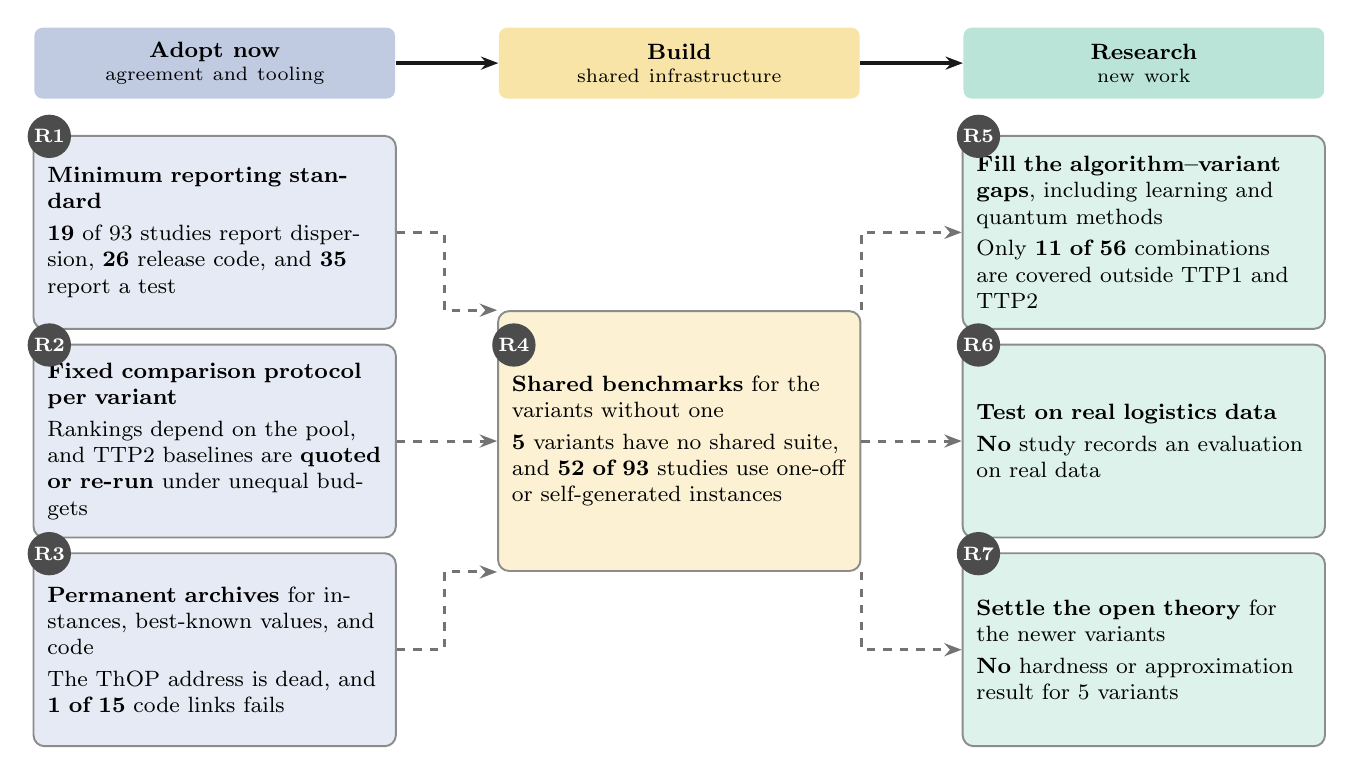
\begin{tikzpicture}[
  font=\footnotesize, >={Stealth[length=2.2mm]},
  ban/.style={draw=none,rounded corners=3pt,align=center,inner sep=4pt,
              minimum height=0.9cm,text width=4.3cm,font=\bfseries\footnotesize},
  rec/.style={draw=black!45,line width=0.7pt,rounded corners=4pt,align=left,
              inner sep=5pt,text width=4.25cm,minimum height=2.45cm,font=\footnotesize},
  badge/.style={circle,draw=none,fill=black!70,text=white,font=\bfseries\scriptsize,
                minimum size=0.55cm,inner sep=0pt},
  flow/.style={->,line width=1.5pt,black!90},
  dep/.style={->,line width=1.1pt,black!55,dashed},
]
\node[ban,fill=VarTTP1!55]  (b1) at (0,0)    {Adopt now\\[-1pt]\normalfont\scriptsize agreement and tooling};
\node[ban,fill=FigAmber!45] (b2) at (5.9,0)  {Build\\[-1pt]\normalfont\scriptsize shared infrastructure};
\node[ban,fill=VarPWT!45]   (b3) at (11.8,0) {Research\\[-1pt]\normalfont\scriptsize new work};
\draw[flow] (b1.east) -- (b2.west);
\draw[flow] (b2.east) -- (b3.west);

\node[rec,fill=VarTTP1!22] (r1) at (0,-2.15) {\textbf{Minimum reporting standard}\\[2pt]
  \textbf{19} of 93 studies report dispersion, \textbf{26} release code, and \textbf{35} report a test};
\node[rec,fill=VarTTP1!22] (r2) at (0,-4.8) {\textbf{Fixed comparison protocol per variant}\\[2pt]
  Rankings depend on the pool, and TTP2 baselines are \textbf{quoted or re-run} under unequal budgets};
\node[rec,fill=VarTTP1!22] (r3) at (0,-7.45) {\textbf{Permanent archives} for instances, best-known values, and code\\[2pt]
  The ThOP address is dead, and \textbf{1 of 15} code links fails};
\node[rec,fill=FigAmber!22,minimum height=3.3cm] (r4) at (5.9,-4.8) {\textbf{Shared benchmarks} for the variants without one\\[2pt]
  \textbf{5} variants have no shared suite, and \textbf{52 of 93} studies use one-off or self-generated instances};
\node[rec,fill=VarPWT!22] (r5) at (11.8,-2.15) {\textbf{Fill the algorithm--variant gaps}, including learning and quantum methods\\[2pt]
  Only \textbf{11 of 56} combinations are covered outside TTP1 and TTP2};
\node[rec,fill=VarPWT!22] (r6) at (11.8,-4.8) {\textbf{Test on real logistics data}\\[2pt]
  \textbf{No} study records an evaluation on real data};
\node[rec,fill=VarPWT!22] (r7) at (11.8,-7.45) {\textbf{Settle the open theory} for the newer variants\\[2pt]
  \textbf{No} hardness or approximation result for 5 variants};

\foreach \n/\x/\y in {1/0/-2.15,2/0/-4.8,3/0/-7.45,4/5.9/-4.8,5/11.8/-2.15,6/11.8/-4.8,7/11.8/-7.45}
  \node[badge] at ($(\x,\y)+(-2.1,1.22)$) {R\n};

\draw[dep] (r1.east) -- ++(0.6,0) |- (r4.north west);
\draw[dep] (r2.east) -- (r4.west);
\draw[dep] (r3.east) -- ++(0.6,0) |- (r4.south west);
\draw[dep] (r4.east) -- (r6.west);
\draw[dep] (r4.north east) |- (r5.west);
\draw[dep] (r4.south east) |- (r7.west);
\end{tikzpicture}}
\caption{Roadmap of the seven recommendations, by tier, with the finding that motivates each. Dashed arrows show dependencies.}
\label{fig:agenda}
\end{figure}

\end{document}
